\documentclass[11pt,letterpaper]{article}
\usepackage[margin=1in]{geometry}
\usepackage{graphicx}
\usepackage{hyperref}
\usepackage{listings}
\usepackage{amsmath}
\pagestyle{headings}
\usepackage{epstopdf}

\begin{document}

\title{PHY 410 \\ Homework Assignment 7}
\author{Han Wen \\ \tiny Person No. 50096432}
\date{\today}

\maketitle

\begin{abstract}
The goal of this assignment was to get familiar with ODE computation and realize the application on non-linear physics.  


\end{abstract}

\tableofcontents

\newpage
\section{Problem 1}

\subsection{Description}

Using inspiration from standard PHY 301-302 Intermediate Mechanics and PHY 509 Classical Dynamics textbooks, generate several trajectories of the nonlinear driven pendulum for the parameters suggested in your mechanics textbook. Generate a bifurcation diagram (as described in class, and here \url{http://en.wikipedia.org/wiki/Bifurcation_diagram}) for a few values of the input strength between 1 and 1.1. Your choice should capture some of the relevant dynamics (i.e. you should have examples of one-cycles, two-cycles, four-cycles, chaotic cycles).

You can also use this reference for inspiration : 

\url{http://www.thphys.uni-heidelberg.de/~gasenzer/index.php?n1=teaching&n2=chaos} 

Hints : (a) You may have to protect against numerical division by zero here (*) for some values of parameters : 

        AvePeriod /= nPeriod\\
   for i in xrange( nPeriod ) :\\
       ErrorBar += (period[i] - AvePeriod)*(period[i] - AvePeriod)\\
   if $nPeriod > 1$ :\\
       ErrorBar = sqrt(ErrorBar/(nPeriod*(nPeriod-1)))\\
   else :\\
       ErrorBar = 0.0\\
   print "Average period = " + str( AvePeriod ) + " +/- " + str( ErrorBar )\\

(b) You should throw away ~100 cycles in the Poincare map to get appropriate dynamics. 

\subsection{Numerical Analysis}

The result is shown in the diagram: Fig. ~\ref{figure1}.
From the plot we can observe the required four phases. With $D_F$ from 1 to about 1.01, it is 1-cycles case; from about 1.01 to about 1.06, it is 2-cycles case; from 1.06 to about 1.07 it is 4-cycles case; from that point on it is chaotic cycles until about 1.08.

\begin{figure}
\begin{center}
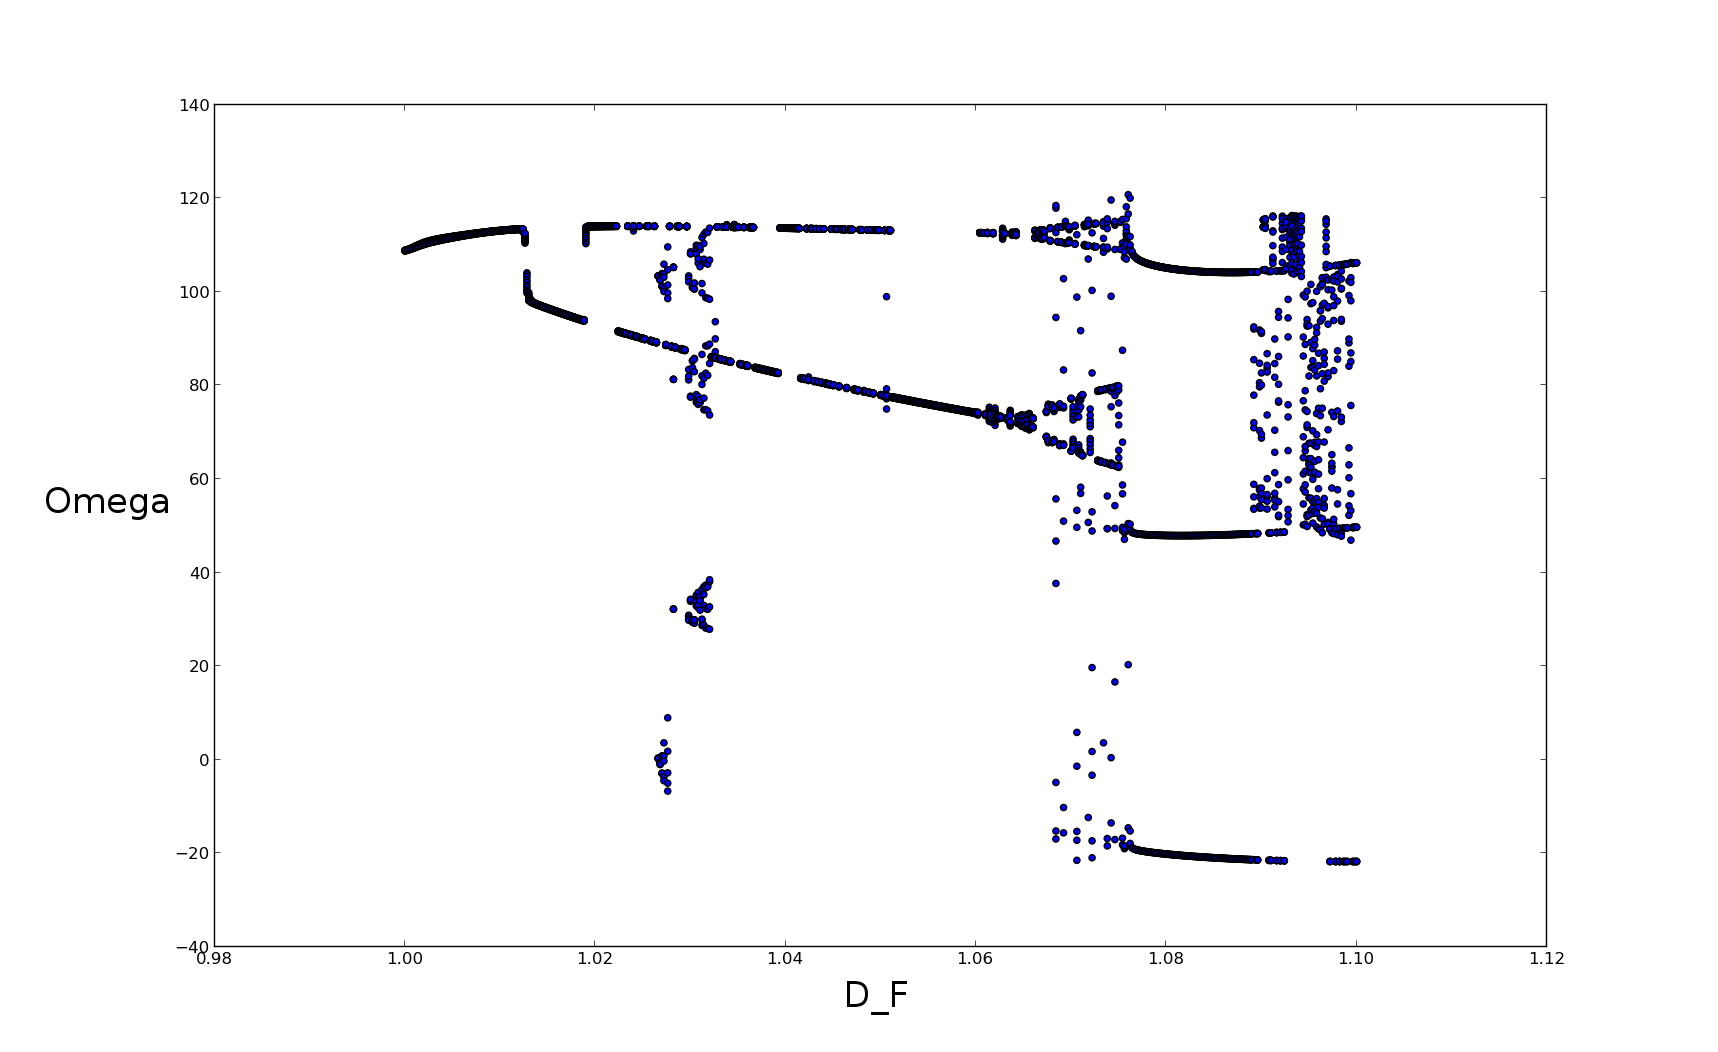
\includegraphics[width=0.8\linewidth,angle=0]{pendulum.png}
\caption{bifurcation}
\label{figure1}
\end{center}
\end{figure}




\newpage

\section{Problem 2}

\subsection{Description}
 In class we considered the Lorenz model : 
 $$
 \frac{dx}{dt}=\sigma(y-x)
 $$
 $$
 \frac{dy}{dt}=x(\rho-z)-y
$$
$$ 
 \frac{dz}{dt}=xy-\beta{z}
$$
 with sigma, rho, and beta constants (chosen as sigma=10, beta=8/3 ,and rho = 28). 

Write software to solve this problem with both the Runge-Kutta 4-th order procedure,  and the RK4 Adaptive stepsize procedure. Compare and contrast the convergence and computational time to solve the problem. Is the adaptive stepsize procedure worthwhile in this case? Also demonstrate the butterfly effect, whereby two very close initial points can diverge after N iterations. Demonstrate this graphically (for instance, by showing the two cycles when they diverge, or by plotting the difference of the trajectories versus the time step). 


\subsection{Result}
Inspired by enormous glorious achievement made by our predecessors with the one of the oldest yet most long-lasting language, Fortran! as well as the ambition to be a qualified computational-physicist, I decide to use Fortran and write the origin code of RK method. Here are the result:\\
For initial coordinates(10,10,10) the diagram: Fig ~\ref{figure2} \\
For initial coordinates(10,10,10.1) the diagram: Fig ~\ref{figure3} \\

\begin{figure}
\begin{center}
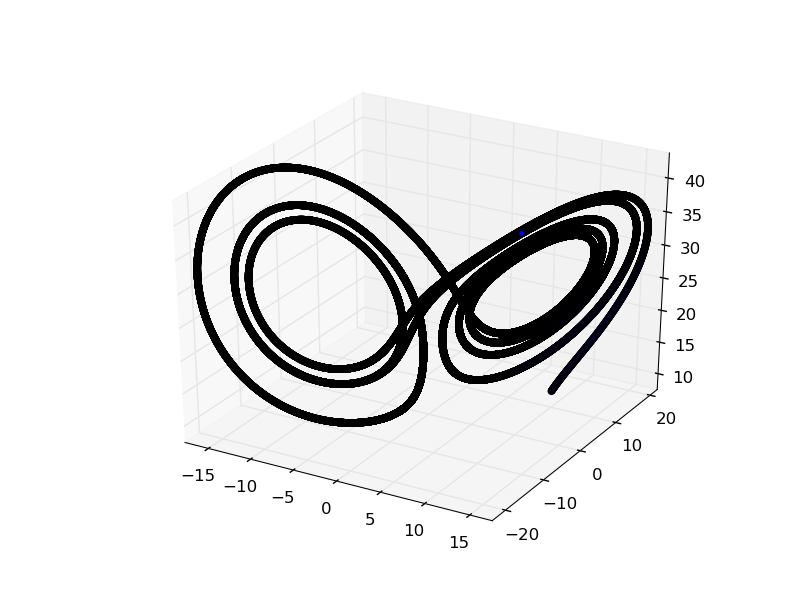
\includegraphics[width=0.8\linewidth,angle=0]{butterfly.png}
\caption{butterfly 10 10 10}
\label{figure2}
\end{center}
\end{figure}

\begin{figure}
\begin{center}
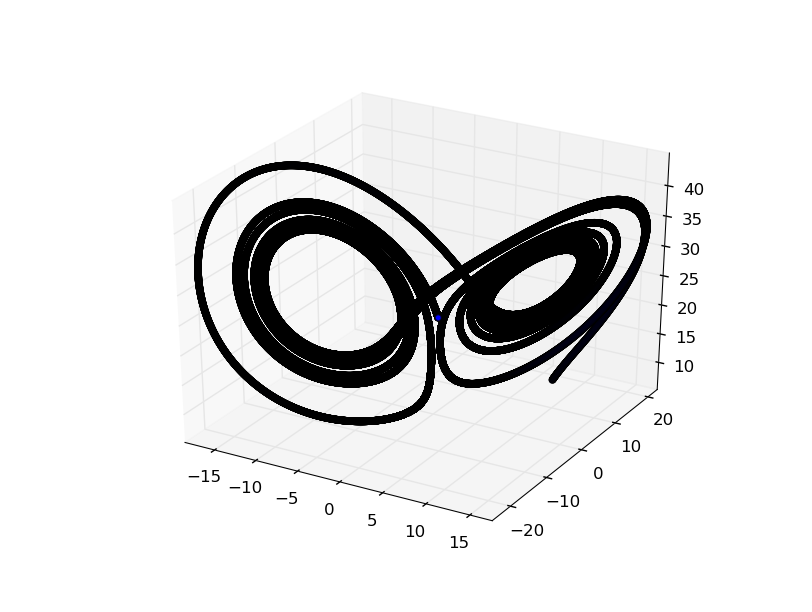
\includegraphics[width=0.8\linewidth,angle=0]{butterfly1.png}
\caption{butterfly 10 10 10.1}
\label{figure3}
\end{center}
\end{figure}

We can see although they two are quite similar, but still fundamentally different. Here is the difference of component vs. time : Fig ~\ref{figure4}

\begin{figure}
\begin{center}
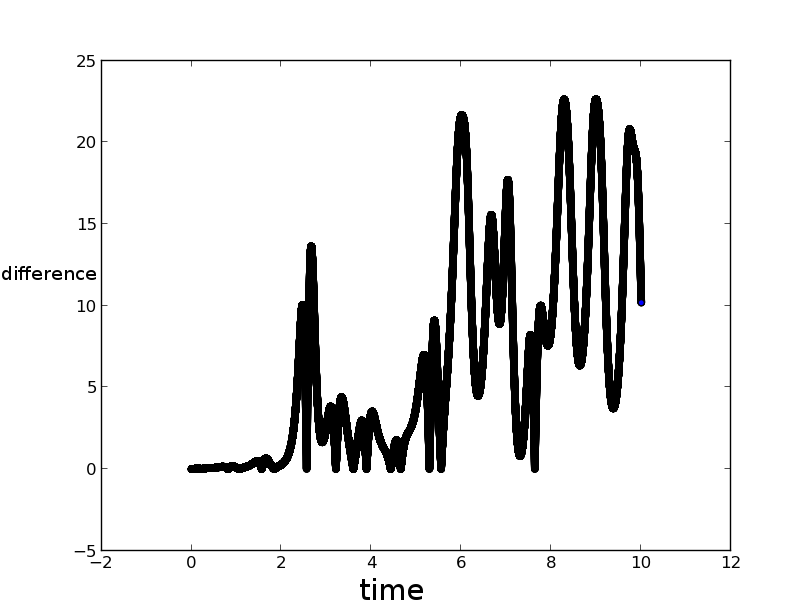
\includegraphics[width=0.8\linewidth,angle=0]{butterflydiff.png}
\caption{difference of x component}
\label{figure4}
\end{center}
\end{figure}

Since I am using Fortran, using adaptive method may not be a good choice and the comparison is somehow pointless. Since for Fortran, as far as I know, floating-point calculation will be much faster than other language while other syntax such as if will not be that fast. To simulate for same amount of time, regular RK-4 method took about 0.33 s, while adaptive method took 3.69 s, despite I gave a rather big accuracy, and consequently it generate much more data. Therefore I should say the adaptive method is not worthwhile and Fortran is a really good language for physicist if they want to do some simple structured yet highly FLoating-point Operational computing.\\
By the way, I think usually the adaptive method is referring to different order of RK method.


\newpage

\section{Problem 3}
\subsection{Description}
Generate the FFT power spectrum for the x, y, and z time series in Problem 2. Plot them. Compare the spectra for similarities and differences. What does this tell you about the behavior of the system? 



\subsection{Result}

Here are the diagram of the fft of x,y,z component vs. time:Fig ~\ref{figure5} ~\ref{figure6} ~\ref{figure7}


\begin{figure}
\begin{center}
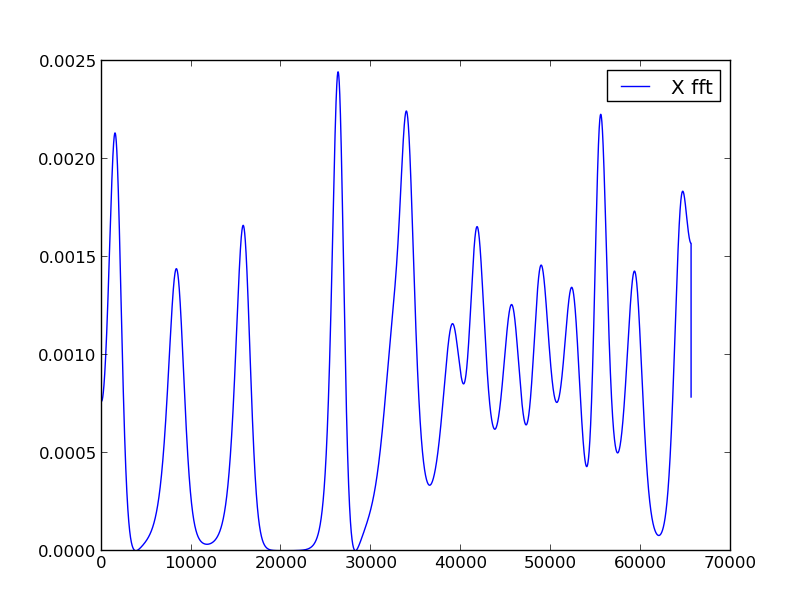
\includegraphics[width=0.8\linewidth,angle=0]{fftx.png}
\caption{FFT power spectrum of x component}
\label{figure5}
\end{center}
\end{figure}

\begin{figure}
\begin{center}
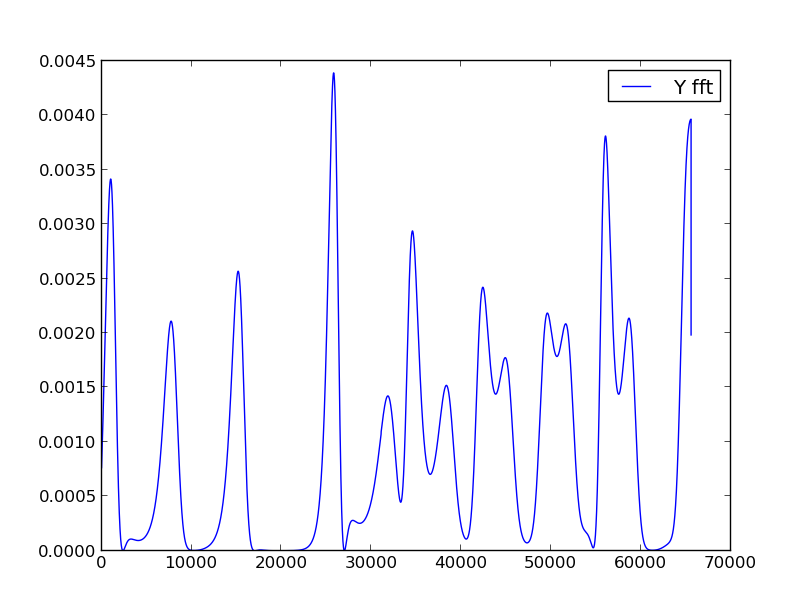
\includegraphics[width=0.8\linewidth,angle=0]{ffty.png}
\caption{FFT power spectrum of y component}
\label{figure6}
\end{center}
\end{figure}

\begin{figure}
\begin{center}
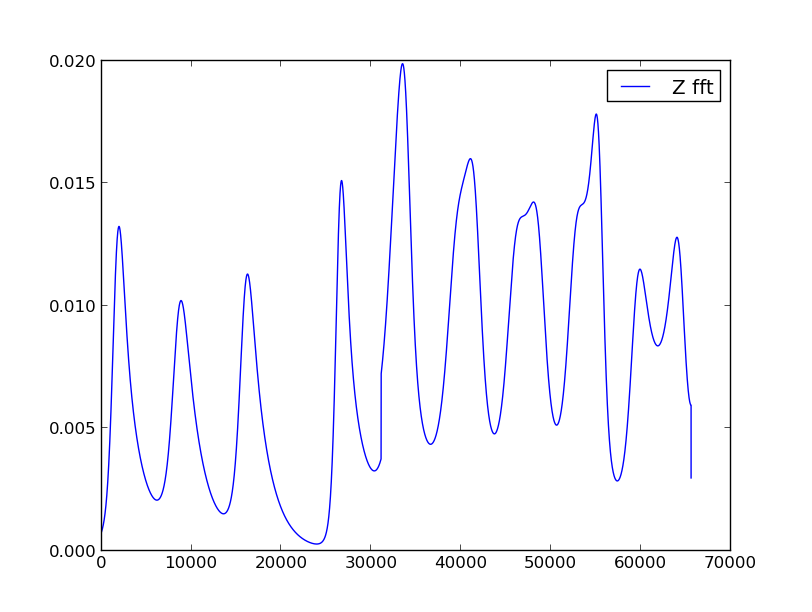
\includegraphics[width=0.8\linewidth,angle=0]{fftz.png}
\caption{FFT power spectrum of z component}
\label{figure7}
\end{center}
\end{figure}

We can see, first of all, these spectra are very similar, going up and down as frequency increases. Yet, they are more or less different in details, especially that of z compared to x and y. This tells us the system distribute the energy with frequency also randomly and differently in different direction, indicating the heterogeneous chaotic behaviour of the system in space.

\newpage
\section*{Acknowledgements}

I discussed this assignment with my classmates and used material from the
cited references, but this write-up is my own.

\begin{thebibliography}{9}


\bibitem{coursepage}
PHY 410-505 Webpage, \url{http://www.physics.buffalo.edu/phy410-505}.



\bibitem{paper}
RK method
\url{http://en.wikipedia.org/wiki/Runge%E2%80%93Kutta_methods#Adaptive_Runge.E2.80.93Kutta_methods}

\bibitem{plot of 2d function}
\url{http://www.thphys.uni-heidelberg.de/~gasenzer/index.php?n1=teaching&n2=chaos}

\end{thebibliography}

\newpage
\appendix
\section{Appendix}

\subsection{c++ fortran python code}

The following python code was used to obtain the results in this report:

\lstinputlisting[language=c++]{pendul_nonlin.cpp}

\lstinputlisting[language=fortran]{lorentz.f90}

\lstinputlisting[language=fortran]{adap.f90}

\lstinputlisting[language=python]{fftbutterfly.py}

\end{document}
